\iffalse
This file is protected by Copyright. Please refer to the COPYRIGHT file
distributed with this source distribution.

This file is part of OpenCPI <http://www.opencpi.org>

OpenCPI is free software: you can redistribute it and/or modify it under the
terms of the GNU Lesser General Public License as published by the Free Software
Foundation, either version 3 of the License, or (at your option) any later
version.

OpenCPI is distributed in the hope that it will be useful, but WITHOUT ANY
WARRANTY; without even the implied warranty of MERCHANTABILITY or FITNESS FOR A
PARTICULAR PURPOSE. See the GNU Lesser General Public License for more details.

You should have received a copy of the GNU Lesser General Public License along
with this program. If not, see <http://www.gnu.org/licenses/>.
\fi

%----------------------------------------------------------------------------------------
% Update the docTitle and docVersion per document
%----------------------------------------------------------------------------------------
\def\docTitle{OpenCPI\\ \bigskip Matchstiq-Z1 Getting Started Guide}
\def\docVersion{1.6}
\def\rccplatform{xilinx13\_3}
\def\radioName{Matchstiq-Z1}
\def\mountPoint{/mnt/}
\def\copyLoc{ATLAS}
%----------------------------------------------------------------------------------------
\def\snippetpath{../../../../../../doc/av/tex/snippets}
% Usage:
% \def\snippetpath{../../../../../doc/av/tex/snippets/}
% % Usage:
% \def\snippetpath{../../../../../doc/av/tex/snippets/}
% % Usage:
% \def\snippetpath{../../../../../doc/av/tex/snippets/}
% \input{\snippetpath/includes}
% From then on, you can use "input" With no paths to get to "snippets"
% You also get all "major" snippets not part of the global LaTeX_Header
% NOTE: If not using the global LaTeX_Header, you need to
% \usepackage{ifthen} to use the \githubio macro

\hyphenation{ANGRY-VIPER} % Tell it where to hyphenate
\hyphenation{Cent-OS} % Tell it where to hyphenate
\hyphenation{install-ation} % Tell it where to hyphenate

\newcommand{\todo}[1]{\textcolor{red}{TODO: #1}\PackageWarning{TODO:}{#1}} % To do notes
\newcommand{\code}[1]{\texttt{#1}} % For inline code snippet or command line
\newcommand{\sref}[1]{Section~\ref{#1}} % To quickly reference a section

% To quickly reference a versioned PDF on gitlab.io
\def\ocpiversion{develop}

% This gives a link to gitlab.io document. By default, it puts the filename.
% You can optionally change the link, e.g.
% \githubio{FPGA\_Vendor\_Tools\_Installation\_Guide.pdf} vs.
% \githubio[\textit{FPGA Vendor Tools Installation Guide}]{FPGA\_Vendor\_Tools\_Installation\_Guide.pdf}
% or if you want the raw ugly URL to come out, \githubioURL{FPGA_Vendor_Tools_Installation_Guide.pdf}
\newcommand{\githubio}[2][]{% The default is for FIRST param!
\href{http://opencpi.gitlab.io/releases/\ocpiversion/docs/#2}{\ifthenelse{\equal{#1}{}}{\texttt{#2}}{#1}}}
\newcommand{\gitlabcom}[2][]{% The default is for FIRST param!
\href{http://gitlab.com/opencpi/#2}{\ifthenelse{\equal{#1}{}}{\texttt{#2}}{#1}}}
\newcommand{\githubioURL}[1]{\url{http://opencpi.gitlab.io/releases/\ocpiversion/docs/#1}}
% Lastly, if you want a SINGLE leading path stripped, e.g. assets/X.pdf => X.pdf:
\newcommand{\githubioFlat}[1]{%
\StrBehind{#1}{/}[\den]%
\href{http://opencpi.gitlab.io/releases/\ocpiversion/docs/#1}{\texttt{\den}}%
}

% Fix import paths
\makeatletter
\def\input@path{{\snippetpath/}}
\makeatother

% From then on, you can use "input" With no paths to get to "snippets"
% You also get all "major" snippets not part of the global LaTeX_Header
% NOTE: If not using the global LaTeX_Header, you need to
% \usepackage{ifthen} to use the \githubio macro

\hyphenation{ANGRY-VIPER} % Tell it where to hyphenate
\hyphenation{Cent-OS} % Tell it where to hyphenate
\hyphenation{install-ation} % Tell it where to hyphenate

\newcommand{\todo}[1]{\textcolor{red}{TODO: #1}\PackageWarning{TODO:}{#1}} % To do notes
\newcommand{\code}[1]{\texttt{#1}} % For inline code snippet or command line
\newcommand{\sref}[1]{Section~\ref{#1}} % To quickly reference a section

% To quickly reference a versioned PDF on gitlab.io
\def\ocpiversion{develop}

% This gives a link to gitlab.io document. By default, it puts the filename.
% You can optionally change the link, e.g.
% \githubio{FPGA\_Vendor\_Tools\_Installation\_Guide.pdf} vs.
% \githubio[\textit{FPGA Vendor Tools Installation Guide}]{FPGA\_Vendor\_Tools\_Installation\_Guide.pdf}
% or if you want the raw ugly URL to come out, \githubioURL{FPGA_Vendor_Tools_Installation_Guide.pdf}
\newcommand{\githubio}[2][]{% The default is for FIRST param!
\href{http://opencpi.gitlab.io/releases/\ocpiversion/docs/#2}{\ifthenelse{\equal{#1}{}}{\texttt{#2}}{#1}}}
\newcommand{\gitlabcom}[2][]{% The default is for FIRST param!
\href{http://gitlab.com/opencpi/#2}{\ifthenelse{\equal{#1}{}}{\texttt{#2}}{#1}}}
\newcommand{\githubioURL}[1]{\url{http://opencpi.gitlab.io/releases/\ocpiversion/docs/#1}}
% Lastly, if you want a SINGLE leading path stripped, e.g. assets/X.pdf => X.pdf:
\newcommand{\githubioFlat}[1]{%
\StrBehind{#1}{/}[\den]%
\href{http://opencpi.gitlab.io/releases/\ocpiversion/docs/#1}{\texttt{\den}}%
}

% Fix import paths
\makeatletter
\def\input@path{{\snippetpath/}}
\makeatother

% From then on, you can use "input" With no paths to get to "snippets"
% You also get all "major" snippets not part of the global LaTeX_Header
% NOTE: If not using the global LaTeX_Header, you need to
% \usepackage{ifthen} to use the \githubio macro

\hyphenation{ANGRY-VIPER} % Tell it where to hyphenate
\hyphenation{Cent-OS} % Tell it where to hyphenate
\hyphenation{install-ation} % Tell it where to hyphenate

\newcommand{\todo}[1]{\textcolor{red}{TODO: #1}\PackageWarning{TODO:}{#1}} % To do notes
\newcommand{\code}[1]{\texttt{#1}} % For inline code snippet or command line
\newcommand{\sref}[1]{Section~\ref{#1}} % To quickly reference a section

% To quickly reference a versioned PDF on gitlab.io
\def\ocpiversion{develop}

% This gives a link to gitlab.io document. By default, it puts the filename.
% You can optionally change the link, e.g.
% \githubio{FPGA\_Vendor\_Tools\_Installation\_Guide.pdf} vs.
% \githubio[\textit{FPGA Vendor Tools Installation Guide}]{FPGA\_Vendor\_Tools\_Installation\_Guide.pdf}
% or if you want the raw ugly URL to come out, \githubioURL{FPGA_Vendor_Tools_Installation_Guide.pdf}
\newcommand{\githubio}[2][]{% The default is for FIRST param!
\href{http://opencpi.gitlab.io/releases/\ocpiversion/docs/#2}{\ifthenelse{\equal{#1}{}}{\texttt{#2}}{#1}}}
\newcommand{\gitlabcom}[2][]{% The default is for FIRST param!
\href{http://gitlab.com/opencpi/#2}{\ifthenelse{\equal{#1}{}}{\texttt{#2}}{#1}}}
\newcommand{\githubioURL}[1]{\url{http://opencpi.gitlab.io/releases/\ocpiversion/docs/#1}}
% Lastly, if you want a SINGLE leading path stripped, e.g. assets/X.pdf => X.pdf:
\newcommand{\githubioFlat}[1]{%
\StrBehind{#1}{/}[\den]%
\href{http://opencpi.gitlab.io/releases/\ocpiversion/docs/#1}{\texttt{\den}}%
}

% Fix import paths
\makeatletter
\def\input@path{{\snippetpath/}}
\makeatother

\iffalse
This file is protected by Copyright. Please refer to the COPYRIGHT file
distributed with this source distribution.

This file is part of OpenCPI <http://www.opencpi.org>

OpenCPI is free software: you can redistribute it and/or modify it under the
terms of the GNU Lesser General Public License as published by the Free Software
Foundation, either version 3 of the License, or (at your option) any later
version.

OpenCPI is distributed in the hope that it will be useful, but WITHOUT ANY
WARRANTY; without even the implied warranty of MERCHANTABILITY or FITNESS FOR A
PARTICULAR PURPOSE. See the GNU Lesser General Public License for more details.

You should have received a copy of the GNU Lesser General Public License along
with this program. If not, see <http://www.gnu.org/licenses/>.
\fi

% Sets OpenCPI Version used throughout all the docs. This is updated by
% scripts/update-release.sh when a release is being made and must not
% be changed manually.
\def\ocpiversion{v2.2.0}

\documentclass{article}
\author{}  % Force author to be blank
\date{OpenCPI Release:\ \ \ocpiversion}  % Force date to be blank and override date with version
\title{OpenCPI\\\docTitle}  % docTitle must be defined before including this file
%----------------------------------------------------------------------------------------
% Paper size, orientation and margins
%----------------------------------------------------------------------------------------
\usepackage{geometry}
\geometry{
  letterpaper,  % paper type
  portrait,     % text direction
  left=.75in,   % left margin
  top=.75in,    % top margin
  right=.75in,  % right margin
  bottom=.75in  % bottom margin
}
%----------------------------------------------------------------------------------------
% Header/Footer
%----------------------------------------------------------------------------------------
\usepackage{fancyhdr} \pagestyle{fancy}  % required for fancy headers
\renewcommand{\headrulewidth}{0.5pt}
\renewcommand{\footrulewidth}{0.5pt}
\lhead{\small{\docTitle}}
\rhead{\small{OpenCPI}}
%----------------------------------------------------------------------------------------
% Various packages
%----------------------------------------------------------------------------------------
\usepackage{amsmath}
\usepackage[page,toc]{appendix}  % for appendix stuff
\usepackage{enumitem}
\usepackage{graphicx}   % for including pictures by file
\usepackage{hyperref}   % for linking urls and lists
\usepackage{listings}   % for coding language styles
\usepackage{pdflscape}  % for landscape view
\usepackage{pifont}     % for sideways table
\usepackage{ragged2e}   % for justify
\usepackage{rotating}   % for sideways table
\usepackage{scrextend}
\usepackage{setspace}
\usepackage{subfig}
\usepackage{textcomp}
\usepackage[dvipsnames,usenames]{xcolor}  % for color names see https://en.wikibooks.org/wiki/LaTeX/Colors
\usepackage{xstring}
\uchyph=0  % Never hyphenate acronyms like RCC
\renewcommand\_{\textunderscore\allowbreak}  % Allow words to break/newline on underscores
%----------------------------------------------------------------------------------------
% Table packages
%----------------------------------------------------------------------------------------
\usepackage[tableposition=top]{caption}
\usepackage{float}
\floatstyle{plaintop}
\usepackage{longtable}  % for long possibly multi-page tables
\usepackage{multicol}   % for more advanced table layout
\usepackage{multirow}   % for more advanced table layout
\usepackage{tabularx}   % c=center,l=left,r=right,X=fill
% These define tabularx columns "C" and "R" to match "X" but center/right aligned
\newcolumntype{C}{>{\centering\arraybackslash}X}
\newcolumntype{M}[1]{>{\centering\arraybackslash}m{#1}}
\newcolumntype{P}[1]{>{\centering\arraybackslash}p{#1}}
\newcolumntype{R}{>{\raggedleft\arraybackslash}X}
%----------------------------------------------------------------------------------------
% Block Diagram / FSM Drawings
%----------------------------------------------------------------------------------------
\usepackage{tikz}
\usetikzlibrary{arrows,decorations.markings,fit,positioning,shapes}
\usetikzlibrary{automata}  % used for the fsm
\usetikzlibrary{calc}      % for duplicating clients
\usepgfmodule{oo}          % to define a client box
%----------------------------------------------------------------------------------------
% Colors Used
%----------------------------------------------------------------------------------------
\usepackage{colortbl}
\definecolor{blue}{rgb}{.7,.8,.9}
\definecolor{ceruleanblue}{rgb}{0.16, 0.32, 0.75}
\definecolor{cyan}{rgb}{0.0,0.6,0.6}
\definecolor{darkgreen}{rgb}{0,0.6,0}
\definecolor{deepmagenta}{rgb}{0.8, 0.0, 0.8}
\definecolor{maroon}{rgb}{0.5,0,0}
%----------------------------------------------------------------------------------------
% Define where to hyphenate
%----------------------------------------------------------------------------------------
\hyphenation{Cent-OS}
\hyphenation{install-ation}
%----------------------------------------------------------------------------------------
% Define Commands & Rename Commands
%----------------------------------------------------------------------------------------
\newcommand{\code}[1]{\texttt{#1}}  % For inline code snippet or command line
\newcommand{\sref}[1]{Section~\ref{#1}}  % To quickly reference a section
\newcommand{\todo}[1]{\textcolor{red}{TODO: #1}\PackageWarning{TODO:}{#1}}  % To do notes
\renewcommand{\contentsname}{Table of Contents}
\renewcommand{\listfigurename}{List of Figures}
\renewcommand{\listtablename}{List of Tables}

% This gives a link to gitlab.io document. By default, it outputs the filename.
% You can optionally change the link, e.g.
% \githubio{FPGA\_Vendor\_Tools\_Installation\_Guide.pdf} vs.
% \githubio[\textit{FPGA Vendor Tools Installation Guide}]{FPGA\_Vendor\_Tools\_Installation\_Guide.pdf}
% or if you want the raw ugly URL to come out, \githubioURL{FPGA_Vendor_Tools_Installation_Guide.pdf}
\newcommand{\githubio}[2][]{% The default is for FIRST param!
\href{http://opencpi.gitlab.io/releases/\ocpiversion/docs/#2}{\ifthenelse{\equal{#1}{}}{\texttt{#2}}{#1}}}
\newcommand{\gitlabcom}[2][]{% The default is for FIRST param!
\href{http://gitlab.com/opencpi/#2}{\ifthenelse{\equal{#1}{}}{\texttt{#2}}{#1}}}
\newcommand{\githubioURL}[1]{\url{http://opencpi.gitlab.io/releases/\ocpiversion/docs/#1}}
% Lastly, if you want a SINGLE leading path stripped, e.g. assets/X.pdf => X.pdf:
\newcommand{\githubioFlat}[1]{%
\StrBehind{#1}{/}[\den]%
\href{http://opencpi.gitlab.io/releases/\ocpiversion/docs/#1}{\texttt{\den}}%
}
%----------------------------------------------------------------------------------------
% VHDL Coding Language Style
% modified from: http://latex-community.org/forum/viewtopic.php?f=44&t=22076
%----------------------------------------------------------------------------------------
\lstdefinelanguage{VHDL}
{
  basicstyle=\ttfamily\footnotesize,
  columns=fullflexible,keepspaces,  % https://tex.stackexchange.com/a/46695/87531
  keywordstyle=\color{ceruleanblue},
  commentstyle=\color{darkgreen},
  morekeywords={
    library, use, all, entity, is, port, in, out, end, architecture, of,
    begin, and, signal, when, if, else, process, end,
  },
  morecomment=[l]--
}
%----------------------------------------------------------------------------------------
% XML Coding Language Style
% modified from http://tex.stackexchange.com/questions/10255/xml-syntax-highlighting
%----------------------------------------------------------------------------------------
\lstdefinelanguage{XML}
{
  basicstyle=\ttfamily\footnotesize,
  columns=fullflexible,keepspaces,
  morestring=[s]{"}{"},
  morecomment=[s]{!--}{--},
  commentstyle=\color{darkgreen},
  moredelim=[s][\color{black}]{>}{<},
  moredelim=[s][\color{cyan}]{\ }{=},
  stringstyle=\color{maroon},
  identifierstyle=\color{ceruleanblue}
}
%----------------------------------------------------------------------------------------
% DIFF Coding Language Style
% modified from http://tex.stackexchange.com/questions/50176/highlighting-a-diff-file
%----------------------------------------------------------------------------------------
\lstdefinelanguage{diff}
{
  basicstyle=\ttfamily\footnotesize,
  columns=fullflexible,keepspaces,
  breaklines=true,                            % wrap text
  morecomment=[f][\color{ceruleanblue}]{@@},  % group identifier
  morecomment=[f][\color{red}]-,              % deleted lines
  morecomment=[f][\color{darkgreen}]+,        % added lines
  morecomment=[f][\color{deepmagenta}]{---},  % Diff header lines (must appear after +,-)
  morecomment=[f][\color{deepmagenta}]{+++},
}
%----------------------------------------------------------------------------------------
% Python Coding Language Style
%----------------------------------------------------------------------------------------
\lstdefinelanguage{python}
{
  basicstyle=\ttfamily\footnotesize,
  columns=fullflexible,keepspaces,
  keywordstyle=\color{ceruleanblue},
  commentstyle=\color{darkgreen},
  stringstyle=\color{orange},
  morekeywords={
    print, if, sys, len, from, import, as, open,close, def, main, for, else,
    write, read, range,
  },
  comment=[l]{\#}
}
%----------------------------------------------------------------------------------------
% Fontsize Notes in order from smallest to largest
%----------------------------------------------------------------------------------------
%    \tiny
%    \scriptsize
%    \footnotesize
%    \small
%    \normalsize
%    \large
%    \Large
%    \LARGE
%    \huge
%    \Huge

\iffalse
This file is protected by Copyright. Please refer to the COPYRIGHT file
distributed with this source distribution.

This file is part of OpenCPI <http://www.opencpi.org>

OpenCPI is free software: you can redistribute it and/or modify it under the
terms of the GNU Lesser General Public License as published by the Free Software
Foundation, either version 3 of the License, or (at your option) any later
version.

OpenCPI is distributed in the hope that it will be useful, but WITHOUT ANY
WARRANTY; without even the implied warranty of MERCHANTABILITY or FITNESS FOR A
PARTICULAR PURPOSE. See the GNU Lesser General Public License for more details.

You should have received a copy of the GNU Lesser General Public License along
with this program. If not, see <http://www.gnu.org/licenses/>.
\fi

\iffalse

This snippet defines macros to be used when describing ocpidev commands
to give the user the equivalent in the IDE. See AV-4628.

To see all output:
\code{\$ ocpidev build something something}
\OcpidevBuild
\code{\$ ocpidev clean something something}
\OcpidevClean
\code{\$ ocpidev run test something something}
\OcpidevRunTest
\code{\$ ocpidev create (no options)}
\OcpidevCreate{}
\code{\$ ocpidev create project}
\OcpidevCreate{Project}
\code{\$ ocpidev clean project Project}
\OcpidevCleanProject{Project}
\code{\$ ocpidev register project my\_proj}
\OcpidevRegisterProject{my_proj}
\code{\$ ocpidev unregister project my\_proj}
\OcpidevUnRegisterProject{my_proj}

\fi
% https://tex.stackexchange.com/a/5227
\usetikzlibrary{shadows}
\newcommand*\OcpidevKeystroke[1]{%
  \tikz[baseline=(key.base)]
    \node[%
      draw,
      fill=white,
      drop shadow={shadow xshift=0.25ex,shadow yshift=-0.25ex,fill=black,opacity=0.75},
      rectangle,
      rounded corners=2pt,
      inner sep=1pt,
      line width=0.5pt,
      font=\scriptsize\sffamily
    ](key) {#1\strut}
  ;
}

\providecommand{\OcpidevCtrlClick}{(use \OcpidevKeystroke{~Ctrl~} for multiple selection)}

\providecommand{\OcpidevTemplate}[1]{
\begin{center}
\framebox{\parbox{0.8\linewidth}{\textit{To perform this operation within the IDE:}
#1}}
\end{center}
}

% OcpidevBuild = "ocpidev build"
\providecommand{\OcpidevBuild}{\OcpidevTemplate{
\begin{enumerate}
\setlength\itemsep{0em} %tighten
\item Open the AV Perspective
\item Select the asset from OpenCPI Project View
\item Import to AV Operations Panel using ``$>$'' button
\item Select the RCC and/or HDL platforms for the build \OcpidevCtrlClick
\item Click ``Build''
\end{enumerate}
}}

% OcpidevClean = "ocpidev clean"
\providecommand{\OcpidevClean}{\OcpidevTemplate{
In the OpenCPI Projects view, select the project, right-click, select clean from the menu.
}}

% OcpidevRunTest = "ocpidev run test"
\providecommand{\OcpidevRunTest}{\OcpidevTemplate{
\begin{enumerate}
\setlength\itemsep{0em} %tighten
\item Click the ``Tests'' radio button and select RCC and/or HDL platforms for the run \OcpidevCtrlClick .
\item Click the ``+remotes'' button, enter the remote string, click OK.
\item Select the remote in the remotes list.
\item In the OpenCPI Projects view, select the desired unit tests, click the ``$>$'' button in the operations panel, then click the desired operation to build and then run the listed tests on the selected remote.
\end{enumerate}
}}

% OcpidevCreate = "ocpidev create <$1>"
\providecommand{\OcpidevCreate}[1]{\OcpidevTemplate{
\begin{itemize}
\setlength\itemsep{0em} %tighten
\item Place the cursor in the OpenCPI Projects panel, right click, select asset wizard.
\item Select the asset type\ifthenelse{\equal{#1}{}}{}{ (``#1'')} in the drop-down, fill in the required inputs, click finish.
\item When the process finishes, the new asset is displayed in both project views. (If the asset has an XML editor, then the editor opens.)
\end{itemize}
}}

% OcpidevCleanProject = "ocpidev clean project <$1>"
\providecommand{\OcpidevCleanProject}[1]{\OcpidevTemplate{\textit{(The project ``#1'' must be imported into the IDE and then refresh the OpenCPI Projects view so the project is shown.)}
\begin{itemize}
\setlength\itemsep{0em} %tighten
\item Right click on #1 $\Rightarrow$ ``Clean''
\end{itemize}
}}

% OcpidevRegisterProject = "ocpidev register project <$1>"
% OcpidevUnRegisterProject = "ocpidev unregister project <$1>"
\providecommand{\OcpidevRegisterProjectKernel}[2]{\OcpidevTemplate{\textit{(The project ``#1'' must be imported into the IDE and then refresh the OpenCPI Projects view so the project is shown.)}
\begin{itemize}
\setlength\itemsep{0em} %tighten
\item In the OpenCPI Projects view, select the project, right-click, select ``#2'' from the menu. (Depending on state of the project, this option may not be available.)
\end{itemize}
}}
\providecommand{\OcpidevRegisterProject}[2]{\OcpidevRegisterProjectKernel{\path{#1}}{register}}
\providecommand{\OcpidevUnRegisterProject}[2]{\OcpidevRegisterProjectKernel{\path{#1}}{unregister}}

\date{Version \docVersion} % Force date to be blank and override date with version
\title{\docTitle}
\lhead{Matchstiq-Z1 Getting Started Guide}
%----------------------------------------------------------------------------------------
\usepackage[T1]{fontenc} % http://tex.stackexchange.com/a/181119
\usepackage{graphicx}
\graphicspath{ {figures/} }
\lstset{ % https://tex.stackexchange.com/a/116572
  basicstyle=\ttfamily,
  columns=fullflexible,
  % frame=single,
  breaklines=true,
  showstringspaces=true,
  showspaces=true,
  postbreak=\mbox{\textcolor{red}{$\hookrightarrow$}\space},
}
\usepackage{textcomp}
\begin{document}
\maketitle
\begin{center}
OpenCPI Release: \ocpiversion
\end{center}
%\thispagestyle{fancy}

\newpage

	\begin{center}
	\textit{\textbf{Revision History}}
		\begin{table}[H]
		\label{table:revisions} % Add "[H]" to force placement of table
			\begin{tabularx}{\textwidth}{|c|X|l|}
			\hline
			\rowcolor{blue}
			\textbf{Revision} & \textbf{Description of Change} & \textbf{Date} \\
		    \hline
            v1.1 & Initial Release & 3/2017 \\
            \hline
            v1.2 & Updated for OpenCPI Release 1.2 & 8/2017 \\
            \hline
            v1.3 & Updated for OpenCPI Release 1.3 & 2/2018 \\
            \hline
            v1.4 & Update descriptions and paths & 9/2018 \\
            \hline
            v1.5 & Update  for OpenCPI Release 1.5 & 4/2019 \\
            \hline
            v1.6 & Refer to installation doc when possible & 1/2020 \\
			\hline
			\end{tabularx}
		\end{table}
	\end{center}

\newpage

\tableofcontents

\newpage

\section{References}
The reference(s) in Table 1 can be used as an overview of OpenCPI and may prove useful.  The installation guide is required since many of the steps mentioned here are defined there, especially in the section:  Enabling OpenCPI Development for Embedded Systems.  This document provides details for this system that can be applied to procedures defined there.  It is best to use both documents at the same time.  This document assumes a basic understanding of the Linux command line (or ``shell'') environment.  
\def\refcapbottom{}
\iffalse
This file is protected by Copyright. Please refer to the COPYRIGHT file
distributed with this source distribution.

This file is part of OpenCPI <http://www.opencpi.org>

OpenCPI is free software: you can redistribute it and/or modify it under the
terms of the GNU Lesser General Public License as published by the Free Software
Foundation, either version 3 of the License, or (at your option) any later
version.

OpenCPI is distributed in the hope that it will be useful, but WITHOUT ANY
WARRANTY; without even the implied warranty of MERCHANTABILITY or FITNESS FOR A
PARTICULAR PURPOSE. See the GNU Lesser General Public License for more details.

You should have received a copy of the GNU Lesser General Public License along
with this program. If not, see <http://www.gnu.org/licenses/>.
\fi

% This snippet creates the "References" table labeled "table:references"
% It creates three columns: Name, Publisher, Link and then inserts default documents
%
% To skip these defaults, define macros named
% refskipgs to skip "Getting Started"
% refskipig to skip "Installation Guide"
% refskipac to skip "Acronyms and Definitions"
% refskipocpiov to skip "OpenCPI Overview"
%
% See RPM_Installation_Guide.tex for examples
%
% After the defaults, it optionally inserts the "myreferences" macro that
% you defined elsewhere (you put hlines above all lines)
%
% If you want the \caption on the bottom, define "refcapbottom"
\begin{center}
\renewcommand*\footnoterule{} % Remove separator line from footnote
\renewcommand{\thempfootnote}{\arabic{mpfootnote}} % Use Arabic numbers (or can't reuse)
\begin{minipage}{0.9\textwidth}
  \begin{table}[H]
\ifx\refcapbottom\undefined
  \caption {References}
  \label{table:references}
\fi
  \begin{tabularx}{\textwidth}{|C|C|}
    \hline
    \rowcolor{blue}
    \textbf{Title} & \textbf{Link} \\
\ifx\refskipocpiov\undefined
    \hline
    OpenCPI User Guide & \githubio{OpenCPI\_User.pdf} \\
\fi
\ifx\refskipac\undefined
    \hline
    Acronyms and Definitions & \githubio{Acronyms\_and\_Definitions.pdf} \\
\fi
\ifx\refskipig\undefined
    \hline
    OpenCPI Installation Guide & \githubio{OpenCPI\_Installation.pdf} \\
\fi
\ifx\myreferences\undefined
\else
    \myreferences
\fi
    \hline
  \end{tabularx}
\ifx\refcapbottom\undefined
\else
  \caption {References}
  \label{table:references}
\fi
  \end{table}
\end{minipage}
\end{center}


\section{Overview}
This document provides steps for configuring a factory provided Epiq Solutions Matchstiq-Z1 SDR with the OpenCPI run-time environment for executing applications. \textbf{Note: Only the Z1 version of the Epiq Solutions Matchstiq product line is supported by OpenCPI.}

\section{Prerequisites}
\begin{flushleft}
  It is assumed that the tasks defined in the ``Enabling OpenCPI Development for Embedded Systems'' section of the \githubio[\textit{OpenCPI Installation Guide}]{OpenCPI\_Installation.pdf} have been successfully performed.
  As mentioned there, support for the Matchstiq Z1 system is based on the \textit{ocpi.assets} built-in project, using the \textit{matchstiq\_z1} OpenCPI HDL (FPGA) platform and the \textit{xilinx13\_3 }OpenCPI RCC (software) platform.  The software platforms are supported by the \textit{ocpi.core} built-in project.

\subsection{Vendor Software Setup}
  Also indicated in the installation guide, the tools used for software cross compilation are from the Xilinx Vivado 2013.4 SDK, and the tools used for the FPGA are any recent version of the Xilinx Vivado Webpack tools.  The Linux Kernel is based on the Xilinx Linux kernel tagged \textit{xilinx-v14.7}.  The installation of these tools is described in the installation guide.

\subsection{Building Required Projects}
\label{sec:Building OpenCPI projects}
The standard built-in OpenCPI projects, as well as the OSP for this system, are built using the above instructions in the installation guide.  This results in a single executable FPGA test application ready to run:  \textit{bias}, based on the \textit{testbias} HDL assembly, both in the \textit{assets} built-in project.

\subsection{Hardware Setup}
\begin{itemize}

\item \textbf{Epiq Solutions Matchstiq-Z1 SDR Kit}\\ \medskip
It is expected that this SDR kit includes a power supply, two SMA/SMB adapters, micro-USB to USB cable, micro-SD card installed internally (expected).

A micro-USB connector on the back of the Matchstiq-Z1 provides access to the serial connection. To expose this micro-USB connector, the two screws in the back plate must be removed.  Historically, this connector's attachment to the PCB has been extremely fragile, \textbf{so be careful when inserting/removing the mating cable}.\\ \medskip

\begin{figure}[ht]
	\centerline{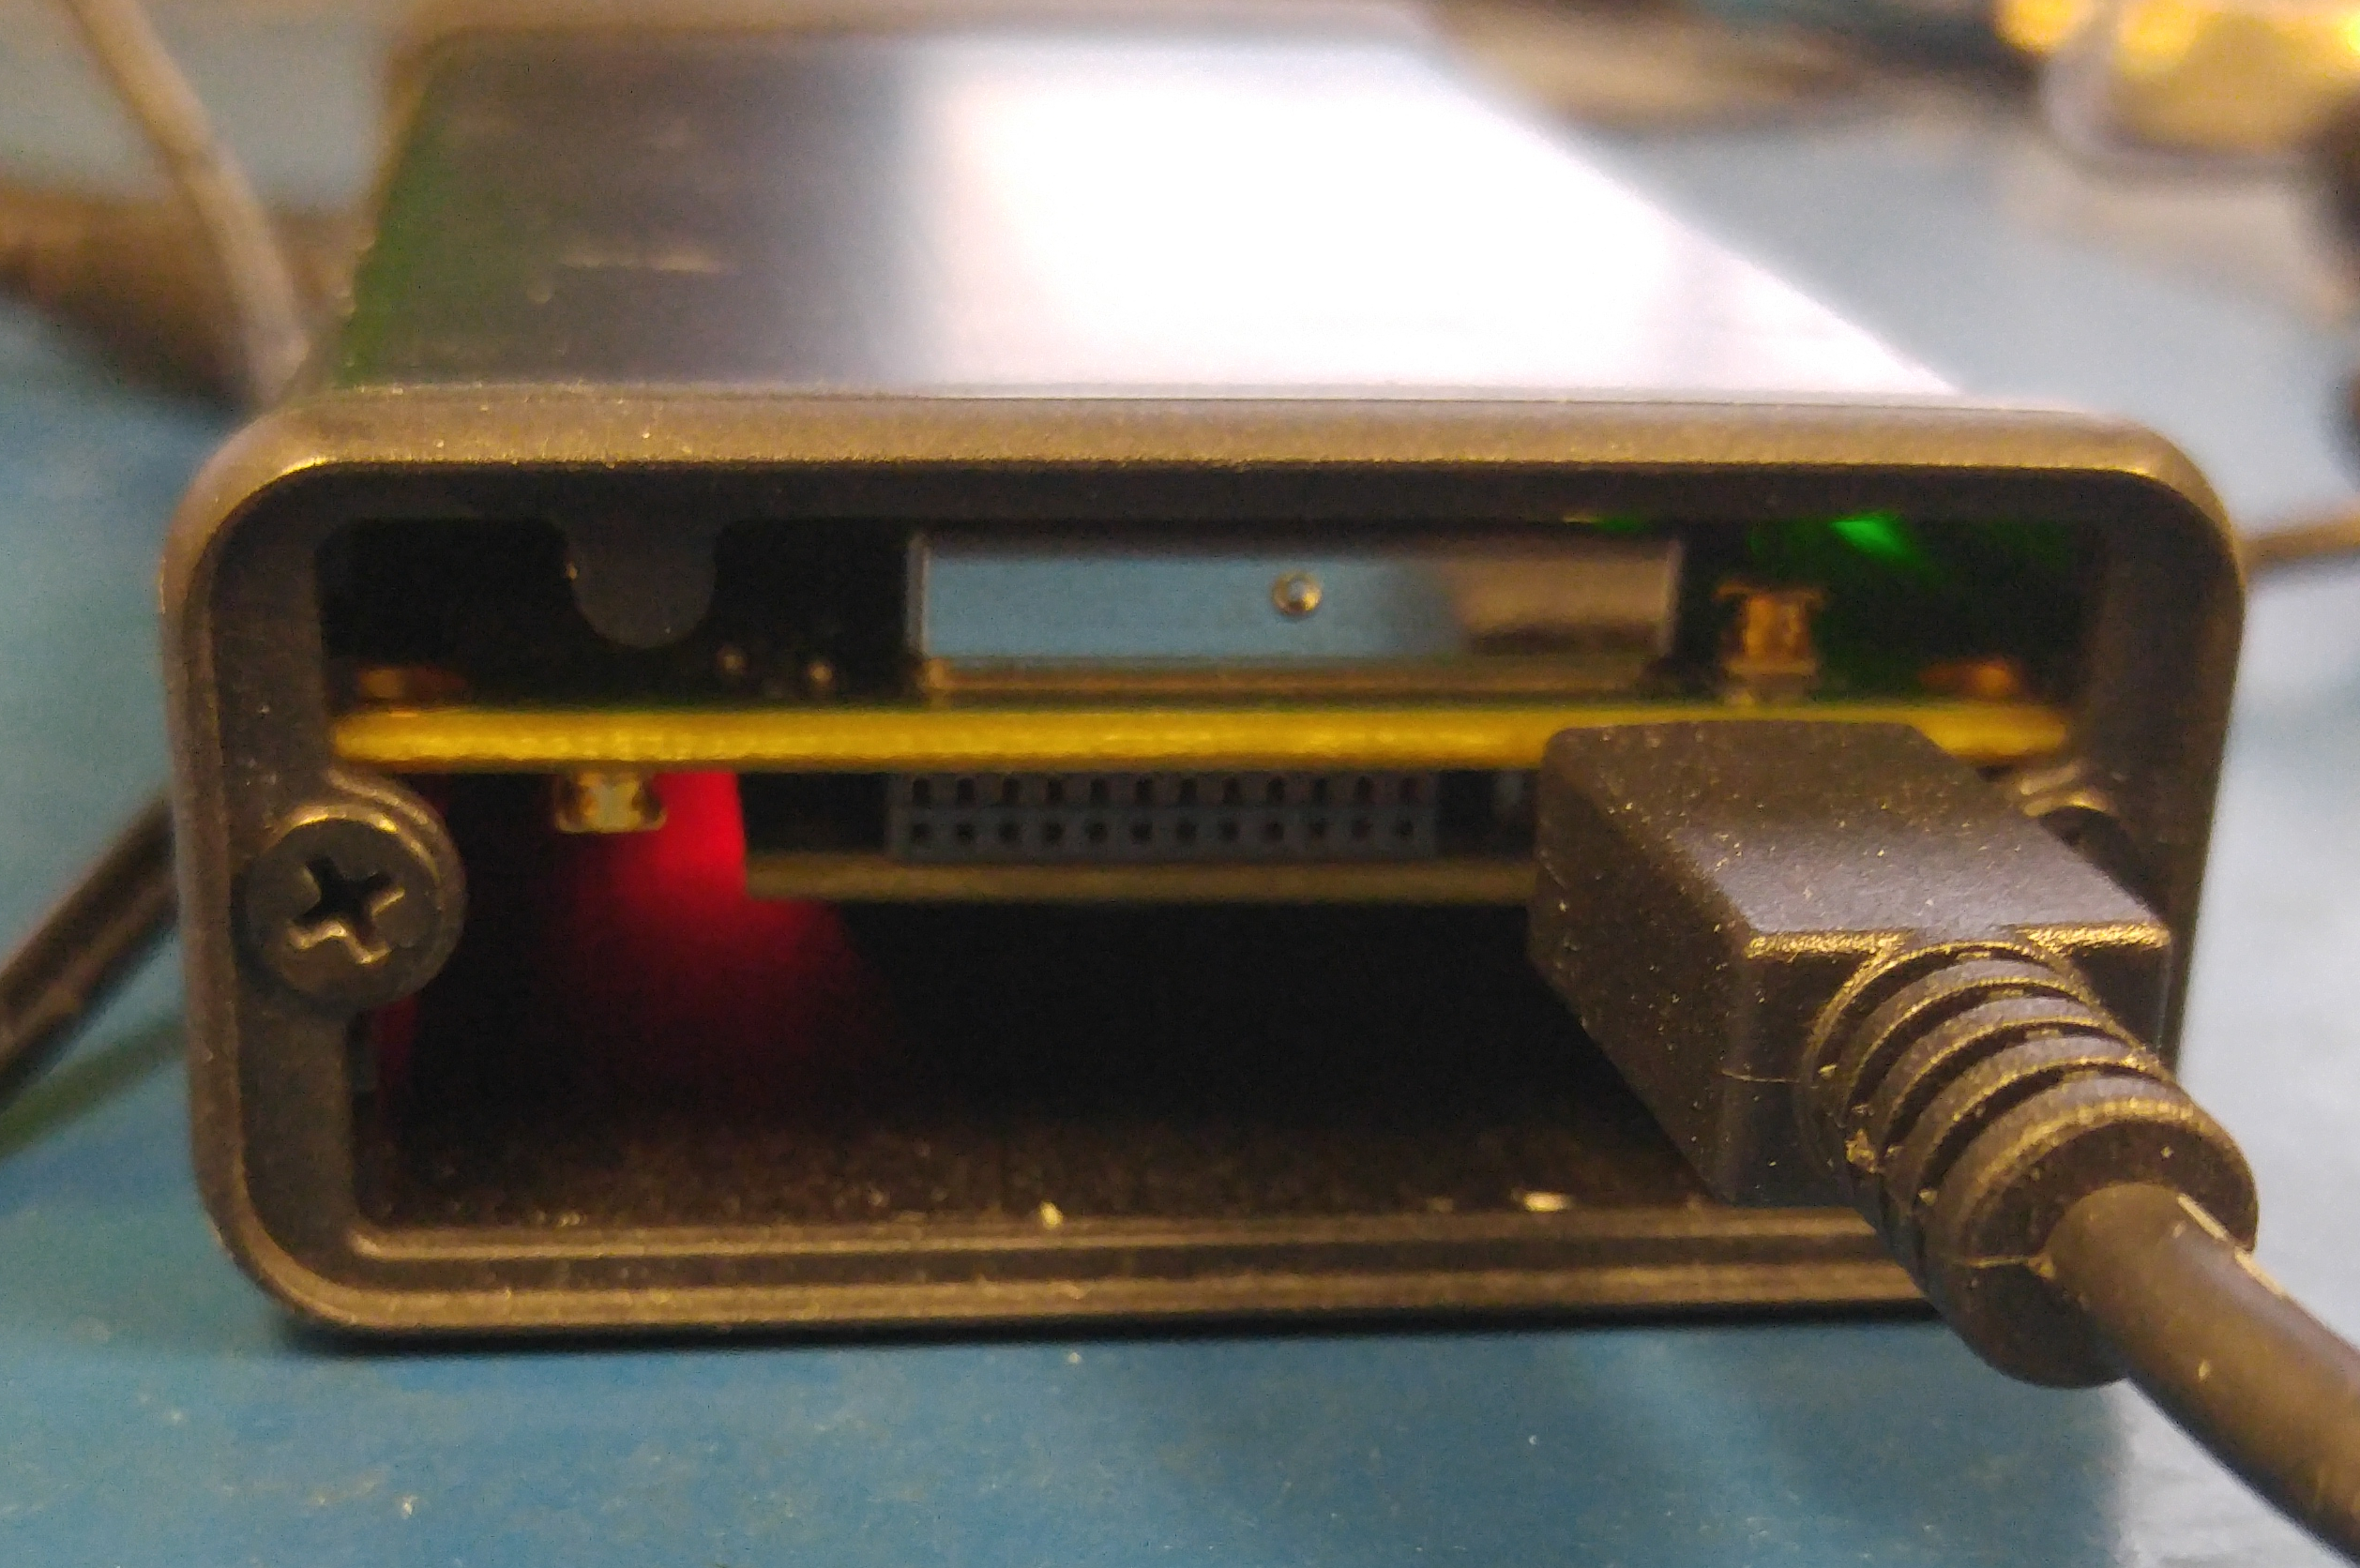
\includegraphics[scale=0.08]{Matchstiq_Z1_backpanel}}
	\caption{Connected Back Panel}
	\label{fig:back}
\end{figure}

\item \textbf{Micro-USB to Ethernet adapter}. To allow network access when plugged into the front panel micro-USB port.  The OpenCPI software platform for the Matchstiq-Z1 is configured for DHCP. An Ethernet connection is required for developing OpenCPI in Network mode.

On the front panel of the Matchstiq-Z1, there are three labeled SMB (50 Ohm) connectors: ``RX'' (receive), ``TX'' (transmit), and ``GPS''.  From the factory, the Matchstiq-Z1 is provided with two SMB to SMA adapters.  Due to the RF performance to the transceiver device, any RF COAX cables should be rated up to at least 3GHz. \\ \medskip
\begin{figure}[ht]
	\centerline{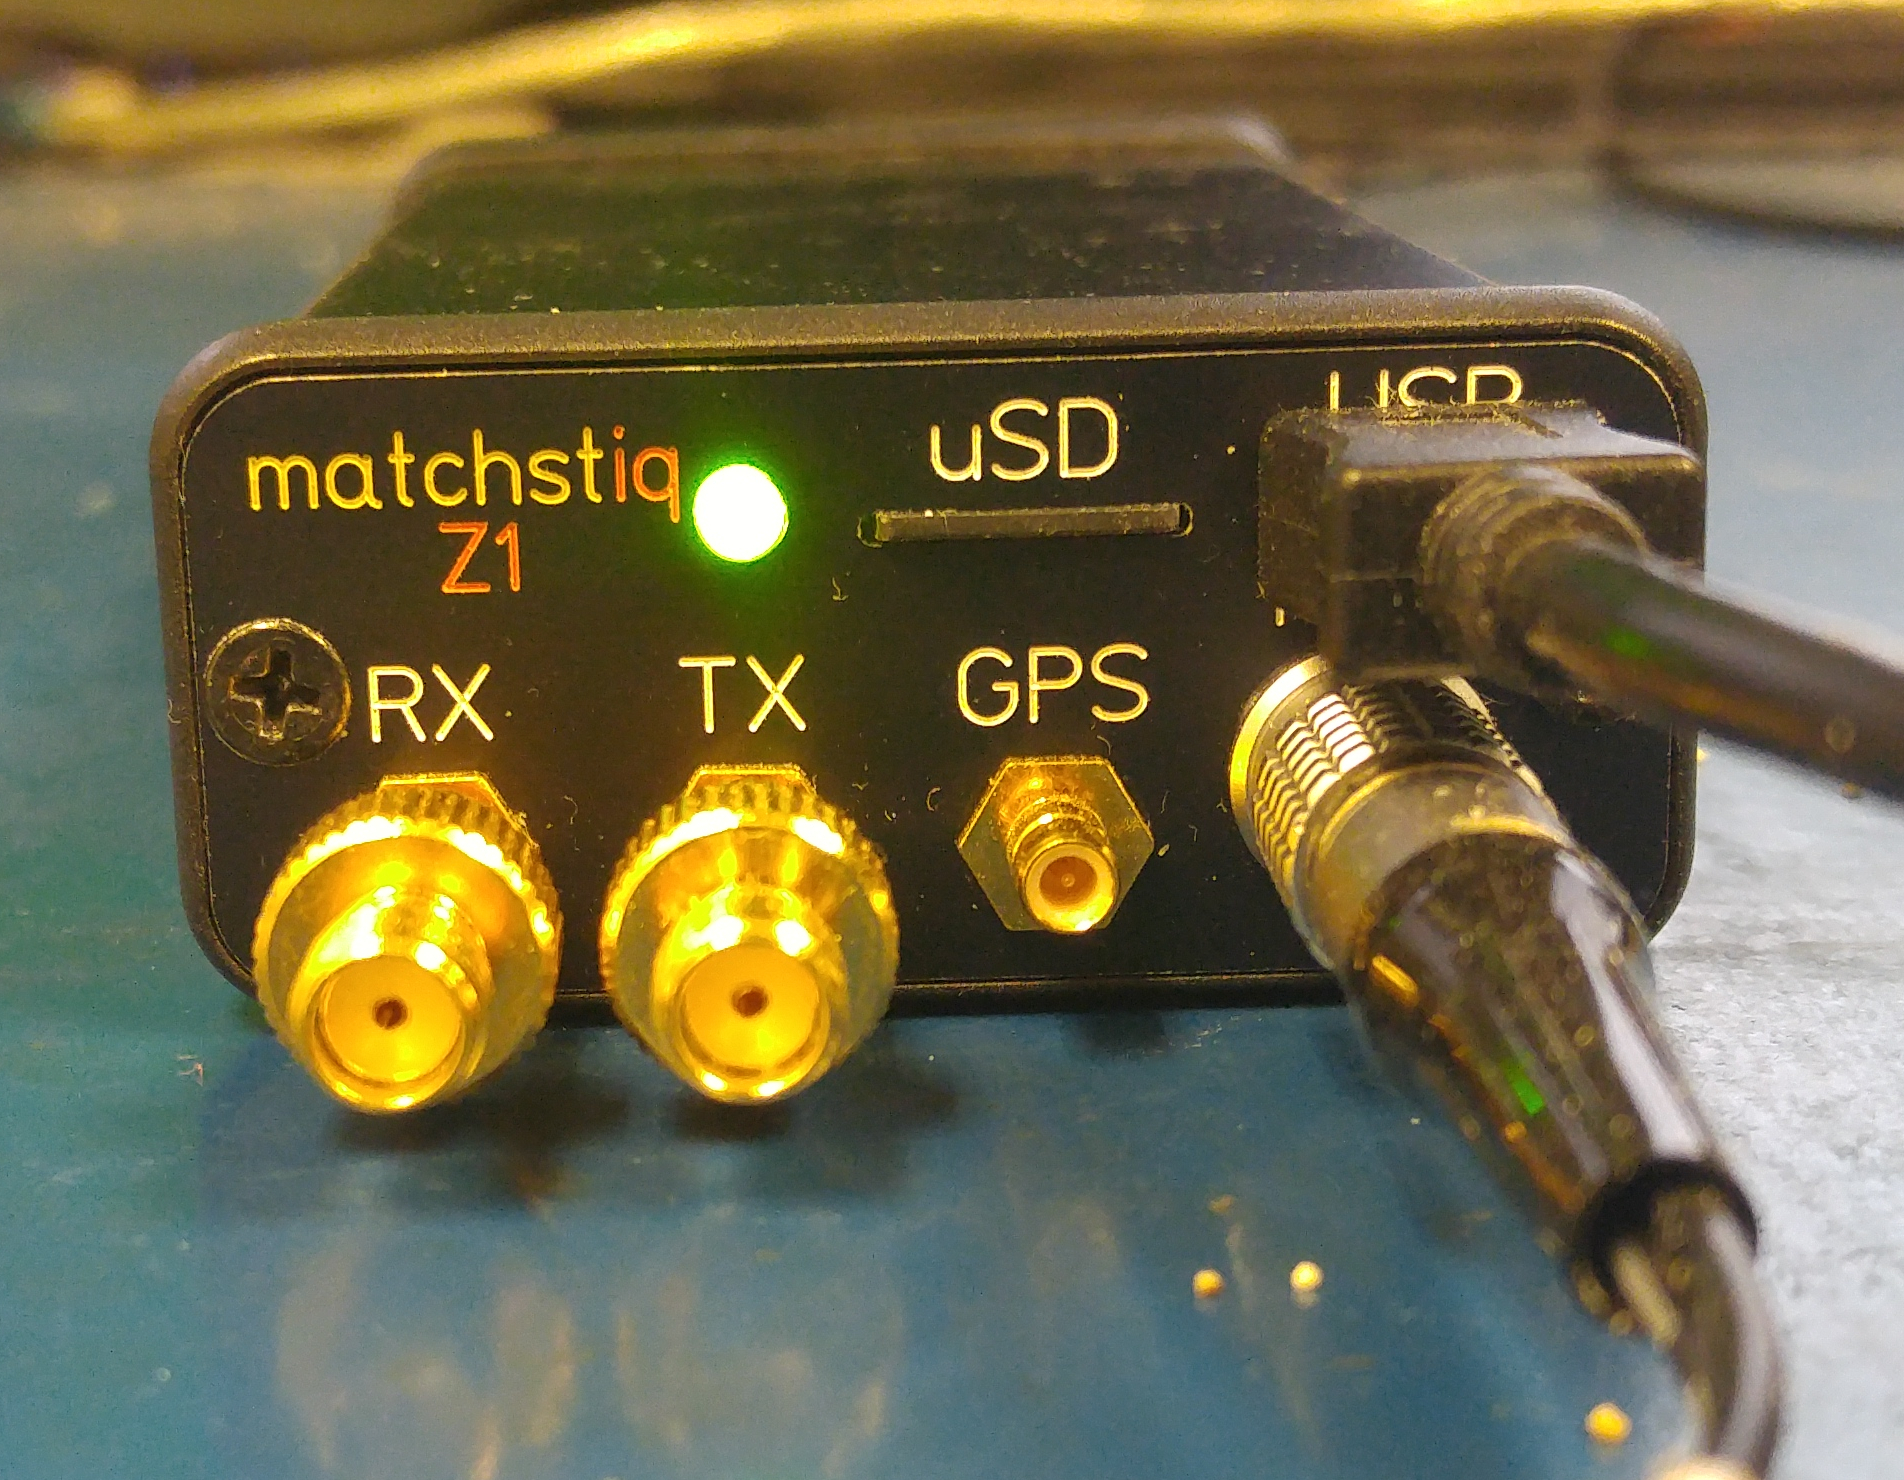
\includegraphics[scale=0.1]{Matchstiq_Z1_frontpanel}}
	\caption{Connected Front Panel}
	\label{fig:front}
\end{figure}

\item \textbf{Access to a network which supports DHCP. (Network Mode)}
\item \textbf{Micro-SD card, 4GB+ (OPTIONAL, as it is possible to use internally installed card) }
\item \textbf{Micro-SD card reader}
\end{itemize}
\end{flushleft}

\newpage
\section{SD Card Setup}
\label{sec:SD_Card_Setup}
The Matchstiq-Z1 SDR is equipped with two SD card slots: one internal and one accessible via the front panel. It is expected that the SDRs are shipped from Epiq Solutions with an SD card installed in the internal slot that is loaded with their embedded environment. A feature of this SDR is that when an SD card is installed in the front panel SD slot, the SDR will automatically choose to operate from this SD card rather than the internal SD card. Therefore, a user can easily switch the SDR between operating in the Epiq Solutions or OpenCPI environment.\\

The Matchstiq-Z1's factory SD card has a non-default formatting and content, which \textit{must} be maintained for proper operation. This guide assumes that the internal (factory) SD card is being use for OpenCPI and will be reinstalled in the front panel SD card slot. If the user desires the use of a new SD card, the user must ensure that it is initially imaged from the factory provided SD card, as there is a unique partition containing required content from the OEM.\\

The installation guide provides the procedure for creating a new SD card for OpenCPI and customizing some of files for your particular configuration.  The usual way is to make a raw copy of the manufacturer supplied card to a new card, preserving formatting and content, and then removing most original files and copying files from OpenCPI.\\

To prepare for OpenCPI provided content to be placed onto the SD card, remove all factory files and directories from the ATLAS partition.  The Matchstiq\_z1 boots from the ``ATLAS'' partition of the SD Card so that is where the OpenCPI contents should be copied.\\

Any files/directories copied to the ``ATLAS'' partition will appear at /mnt/card on the Matchstiq-Z1.\\

All the files in this partition can be ignored. If space for files is required for your application, they can be deleted.

\pagebreak
\section{Hardware Setup}

\subsection{Establish a Serial Connection}
The installation guide provides the procedure establishing a serial console.  On these systems the console serial port operates at 115200 baud.  The cable used is a micro-USB to USB-A cable to connect its  console micro-USB port to the development host.  Remember the micro-USB socket on the Matchstiq Z1 is \textbf{delicate!}.
\subsection{Update U-boot Variables}
\begin{enumerate}
\item Remove power from the Matchstiq-Z1 unit.
\item Insert the SD card into the front panel SD card slot.
\item Connect a terminal to the rear micro-USB connector of the Matchstiq-Z1 with a baud rate of 115200.
\item Apply power to the Matchstiq-Z1 with the terminal still connected and stop the boot process by hitting any key to enter the U-Boot terminal.
\item Run the following commands to setup the environment variables:
\begin{itemize}
\item \texttt{setenv bootcmd \textquotesingle ivmmc; run ocpiboot\textquotesingle}
\item \texttt{setenv ocpiboot \textquotesingle setenv bootargs console=ttyPS0,115200n8 root=/dev/ram rw earlyprintk; \\
setenv fdt\_high ffffffff; setenv initrd\_high 0x1000000; fatload mmc \$\{iv\_mmc\} \$\{dtbaddr\}\\
\$\{dtbfile\}; fatload mmc \$\{iv\_mmc\} \$\{loadaddr\} \$\{bootfile\}; fatload mmc \$\{iv\_mmc\}\\
0x2000000 uramdisk.image.gz; bootm \$\{loadaddr\} 0x2000000 \$\{dtbaddr\}\textquotesingle}
\subitem *Note: This should be a one-line command. Make sure there are no newlines.
\item \texttt{saveenv}
\end{itemize}
\item These U-Boot environment variables are now saved to the second partition of the SD card
\end{enumerate}

\begin{flushleft}
Verify that the changes are correct by running the command ``\texttt{env p}'' and comparing to:
\end{flushleft}
\begin{verbatim}
baudrate=115200
bootcmd=ivmmc;run ocpiboot
bootdelay=3
bootfile=uImage
defargs=setenv bootargs console=ttyPS0,115200n8 mem=240M iv_mb=${iv_mb} iv_io=${iv_io}
iv_bp=${iv_bp} iv_mmc=${iv_mmc} ${otherargs}
dtbaddr=0x02a00000
dtbfile=iveia-atlas-i-z7e.dtb
iv_io=205-00034-00-A0,,Atlas-II_GF_Carrier
iv_io_default=205-00034-00-A0,,Atlas-II_GF_Carrier
iv_io_ord=00034
iv_mb=205-00049-00-B1,A2WT9,Atlas-I-Z7e
iv_mb_ord=00049
iv_mmc=0
loadaddr=0x03000000
mmcdtload=fatload mmc ${iv_mmc} ${dtbaddr} ${dtbfile};fdt addr ${dtbaddr};fdt set
/chosen bootargs "${bootargs}";fdt ivclean ${iv_mb_ord}
mmcxload=axi_reset 1; fatload mmc ${iv_mmc} ${loadaddr} ${xloadfile};xload ${loadaddr}
${filesize}; axi_reset 0;
ocpiboot=setenv bootargs console=ttyPS0,115200n8 mem=240M root=/dev/ram rw earlyprintk;
setenv fdt_high ffffffff;  setenv initrd_high 0x1000000; fatload mmc ${iv_mmc} ${dtbaddr}
${dtbfile}; fatload mmc ${iv_mmc} ${loadaddr} ${bootfile};  fatload mmc ${iv_mmc} 0x2000000
uramdisk.image.gz; bootm ${loadaddr} 0x2000000 ${dtbaddr}
sdboot=run mmcxload;run defargs;fatload mmc ${iv_mmc} ${loadaddr} ${bootfile};run
mmcdtload;setenv fdt_high ffffffff;bootm ${loadaddr} - ${dtbaddr}
stderr=serial
stdin=serial
stdout=serial
xloadfile=xilinx.bit

Environment size: 1283/131068 bytes
\end{verbatim}

\pagebreak
\section{Configuring the runtime environment on the system}
The installation guide provides the procedure for setting up and verifying the runtime environment.
This system is initially set with  ``\textbf{root}'' for user name and password.
After a successful boot to PetaLinux, login to the system, using  ``\textbf{root}`` for user name and password.

\begin{figure}[H]
	\centerline{\includegraphics[scale=0.5]{Matchstiq_Z1_login}}
	\caption{Successful Boot to PetaLinux}
	\label{fig:boot1}
\end{figure}

\section{Run an Application}
See the installation guide for running a small test application.
\pagebreak
\begin{appendices}

\section{Intermittent Errors}
Some tests have had ``Segmentation Faults'' or ``Alignment Errors'' in certain scenarios on the Z1. This seems to happen when both USB ports are used to simultaneously transmit a large amount of data, \textit{e.g.} high log-level output to a USB serial console as well as NFS-mounted output files over a USB-to-Ethernet adapter. The default test setup avoids triggering this by limiting output that is fed to the user, but users should be aware of this issue if non-default test scenarios are attempted. If \texttt{ssh} is used to have all data routed through the USB-to-Ethernet adapter, this failure mode is avoided.
\section{Using ISE instead of Vivado with the Matchstiq-Z1}
It is recommended that you use the default toolset (Xilinx Vivado) to build Matchstiq-Z1 bitstreams with OpenCPI. However, if you wish to use ISE instead, reference the README file in \path{assets/hdl/platforms/matchstiq_z1/ise_constraints/}, and perform the following steps:
\begin{enumerate}
\item{Modify the target part in \path{assets/hdl/platforms/matchstiq_z1/matchstiq_z1.mk} to use the ISE alias:
\subitem \code{HdlPart\_matchstiq\_z1=xc7z020\_ise\_alias-1-clg484}}
\item{Export the ISE constraints files found in \path{<assets/>hdl/platforms/matchstiq_z1/ise_constraints/} by modifying \code{ExportFiles} variable in \path{assets/hdl/platforms/matchstiq_z1/Makefile}:
\subitem \code{ExportFiles=ise\_constraints/matchstiq\_z1.ucf ise\_constraints/matchstiq\_z1.ut matchstiq\_z1.mk}}
\end{enumerate}
% Bring in the kernel message snippet
\section{Driver Notes}
\input{Driver_Snippet}
%
\end{appendices}
\end{document}
